\documentclass[journal,10pt]{IEEEtran}
\usepackage[T1]{fontenc}
\usepackage[utf8]{inputenc}
\usepackage{amsmath,amssymb,graphicx,booktabs,array,cite}
\usepackage[hidelinks]{hyperref}
\graphicspath{{figures/}}
\newcommand{\GaO}{\ensuremath{\beta\text{-}\mathrm{Ga}_2\mathrm{O}_3}}
\newcommand{\pGaN}{\ensuremath{p\text{-}\mathrm{GaN}}}
\newcommand{\Vop}{\ensuremath{V_{\mathrm{BR,op}}}}
\newcommand{\Von}{\ensuremath{V_{\mathrm{on},1}}}
\newcommand{\Ron}{\ensuremath{R_{\mathrm{on,sp}}}}

\title{Geometry and p-GaN Design Sensitivity in \texorpdfstring{$\beta$-Ga$_2$O$_3$}{beta-Ga2O3} Rectifiers: An Axisymmetric TCAD Study}
\author{Harikrishnan}
\begin{document}
\maketitle

\begin{abstract}
We use axisymmetric drift--diffusion simulations to compare planar, mesa, and trench \pGaN{} terminations in \GaO{} rectifiers. The planar junction termination extension and mesa junction-barrier design with field plates reach approximately 2336~V at a reverse-current criterion of 1~mA/cm$^2$, compared with 1133~V for the tested trench design and 929~V for the selected bare reference. In the planar design, increasing the \pGaN{} thickness from 150 to 250~nm or increasing the prescribed acceptor concentration by 50\% reduces the crossing below 700~V. At 400~K, the planar and mesa crossings separate at 1~mA/cm$^2$ but lie close together at 10~mA/cm$^2$. The 80-nm, 0.75-eV planar variant has a turn-on voltage of 0.355~V at 1~A/cm$^2$, but its reverse crossing falls from 2347 to 925~V when the current criterion is tightened to 0.1~mA/cm$^2$. The results describe sensitivities of the simulated structures, not fabrication tolerances or device ratings.
\end{abstract}

\begin{IEEEkeywords}
\GaO, \pGaN, junction termination extension, junction barrier Schottky diode, device simulation.
\end{IEEEkeywords}

\section{Introduction}
Vertical \GaO{} rectifiers are attractive for high-voltage switching, but the absence of a shallow \GaO{} acceptor means that edge termination has to be built from a different material. Yang \emph{et al.} reported unterminated 105-$\mu$m Schottky rectifiers with a mean breakdown voltage of $975\pm40$~V and showed that the blocking voltage falls for larger contact diameters~\cite{Yang2017}. That result provides a reference for the unterminated case and sets the scale against which a termination has to be judged.

\pGaN{} grown or sputtered on \GaO{} supplies the missing p-type region. It can be used as a lateral junction termination extension (JTE), as junction-barrier Schottky (JBS) rings inside the active area, or as both together with a field plate (FP). Simulated \pGaN/\GaO{} JBS structures have been reported~\cite{Nandi2021_TED,Than2024_PhysScr}, and experimental devices now include a 3-kV sputtered-\pGaN{} JTE diode~\cite{Chang2025_APL} and a 4.3-kV \pGaN{} heterojunction-barrier rectifier~\cite{Chang2026_TED}. Low-barrier anodes are also of interest, since a NiO/\GaO{} JBS diode combining a 0.64-V turn-on with 2.34-kV blocking has been demonstrated~\cite{Su2024_APL}.

This study compares planar, raised-ring and recessed-ring \pGaN{} designs in a common axisymmetric framework. We examine how the forward and reverse characteristics change with geometry, prescribed acceptor concentration, Schottky barrier and temperature, and how the choice of reverse-current criterion affects the comparison. Published devices provide context rather than a common-criterion performance ranking.

\section{Simulation Model}
\subsection{Transport and material parameters}
The simulations use Sentaurus Device V-2024.03~\cite{Sentaurus2024} in cylindrical coordinates with Fermi statistics, doping-dependent mobility and high-field velocity saturation. Incomplete ionisation is applied to the donor species in \GaO{} and to Mg in GaN. The Mg activation model uses $E_0=0.20$~eV with a concentration-dependent coefficient of $8.0\times10^{-9}$~eV\,cm and a degeneracy factor of 4, giving 4.0--6.9\% ionised acceptors at 298~K across the three zones; the ionised fraction rises towards unity where the layer is depleted under reverse bias. Thermionic transport is enabled at the GaN/\GaO{} interface, and the interface is treated with a fixed sheet charge of $-2.67\times10^{11}$~cm$^{-2}$ at the \GaO/Al$_2$O$_3$ boundary. Ambient regions are represented as an ideal dielectric with $\varepsilon_r=1$, matching the reference diode, whose characteristics were measured unpassivated in air on a probe station~\cite{Yang2017}; the 298 and 350~K simulations lie inside that measured 25--100~$^\circ$C window, and 400~K lies above it.

The nominal Schottky work function is 5.10~eV, giving a 1.10-eV input barrier against the \GaO{} electron affinity of 4.00~eV. The simulations include image-force barrier lowering and nonlocal electron tunnelling with an effective mass of $0.38m_0$ and a 15-nm path length. The reported architecture and sweep results use a tunnelling prefactor $g=1.56\times10^{-8}$.

\begin{table}[!t]
\caption{Reverse-Transport Parameters Used in the Simulations}
\label{tab:model}
\centering\footnotesize
\begin{tabular}{lll}
\toprule
Quantity & \GaO & GaN\\
\midrule
$a_e$ (cm$^{-1}$) & $7.90\times10^5$ & $2.90\times10^8$\\
$a_h$ (cm$^{-1}$) & $7.90\times10^5$ & $5.41\times10^6$\\
$b_e$ (V/cm) & $2.92\times10^7$ & $3.40\times10^7$\\
$b_h$ (V/cm) & $5.00\times10^7$ & $1.96\times10^7$\\
$\hbar\omega$ (eV) & 0.063 & 0.066\\
\bottomrule
\end{tabular}
\par\smallskip\begin{minipage}{0.98\columnwidth}\footnotesize
The coefficients enter $\alpha=\gamma a\exp(-\gamma b/F)$, with $F$ the quasi-Fermi-gradient driving force and $\gamma$ the temperature factor of the van Overstraeten model.
\end{minipage}
\end{table}

Impact ionisation uses the van Overstraeten form with the quasi-Fermi gradient as the driving force, so the plotted electrostatic field is not by itself a multiplication criterion. The \GaO{} electron coefficients use the $x$-direction fit of Ghosh and Singisetti~\cite{Ghosh2018_JAP} as a scalar model input. The \GaO{} hole coefficients are assumed, and the GaN coefficients are model inputs for the \pGaN{} film (Table~\ref{tab:model}). The \GaO{} permittivity is taken as $12.4\varepsilon_0$, the static value perpendicular to (001), applied as a scalar~\cite{Fiedler2019_ECS}.

The terminated reverse decks include a constant optical generation of $10^{13}$~cm$^{-3}$s$^{-1}$ for numerical stabilisation. For a 10-$\mu$m drift layer, the direct-generation current scale $qGd$ is $1.6\times10^{-9}$~A/cm$^2$ before multiplication, well below the operational current criterion.

\subsection{Numerical sensitivity}
\begin{figure}[!t]
\centering
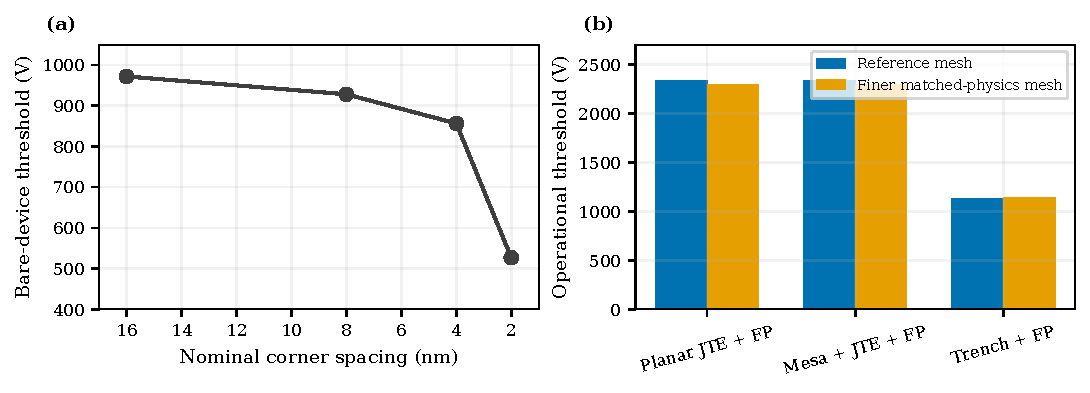
\includegraphics[width=\columnwidth]{numerical_sensitivity.pdf}
\caption{Numerical sensitivity: (a) bare-diode blocking voltage versus nominal corner mesh spacing; (b) blocking-voltage changes across the two meshes tested for each terminated design.}
\label{fig:mesh}
\end{figure}

Figure~\ref{fig:mesh} shows that the bare-diode crossing changes from 972 to 527~V as the nominal corner spacing decreases from 16 to 2~nm in the mesh study. The reported 928.7~V reference is extracted from a separate split-anode current trace at the nominal refinement level used for the architecture comparison. The neighboring single-anode field output is not used to interpret that trace. The terminated-device values reported here are results on the meshes used, not mesh-converged limits.

\subsection{Extraction definitions}
All current densities use the same reference area,
\begin{equation}
A_{\mathrm{ref}}=\pi(52.5\times10^{-4})^2=8.6590\times10^{-5}\ \mathrm{cm}^2 .
\end{equation}
This is a common reference area, not the exposed Schottky area of each device or the total chip area. Terminal current is taken from the cathode. Forward voltage is the external terminal voltage difference; reverse voltage is the magnitude of the anode external potential minus the cathode internal potential.

Blocking is defined at $|J_R|=1$~mA/cm$^2$, i.e. $|I_R|=8.659\times10^{-8}$~A, with logarithmic interpolation between accepted samples. An isolated excursion that returns below the criterion is not accepted; the admitted crossing has to remain above it for the following five samples. Convergence-failure endpoints and sweeps that end without a crossing are not reported as blocking voltages. The reverse sweeps use a separate cathode stop criterion of 1~mA total current, corresponding to about 11.5~A/cm$^2$ on $A_{\mathrm{ref}}$. Turn-on $\Von$ is defined at $J_F=1$~A/cm$^2$, and the higher-current voltage $V_{F,100}$ at 100~A/cm$^2$. Specific resistance is the slope $dV_F/dJ_F$ fitted over 200--300~A/cm$^2$.

Two figures of merit are kept separate:
\begin{align}
M_{\mathrm{on}}&=\frac{V_{\mathrm{BR,op}}^2}{V_{\mathrm{on},1}} &&[\mathrm{V}],\\
B&=\frac{V_{\mathrm{BR,op}}^2}{R_{\mathrm{on,sp}}} &&[\mathrm{W/cm}^2].
\end{align}
Equation (2) addresses the blocking/turn-on objective; (3) is the conventional Baliga metric. They have different units and need not select the same structure.

\section{Device Structures}
Fig.~\ref{fig:structures} shows schematic cross-sections of the four representative geometries. The seven electrical cases are a bare Schottky diode; a planar JTE with and without an FP; a mesa JBS with JTE, with and without an FP; and a trench JBS with JTE, with and without an FP. The trench cases retain the outer three-zone JTE and are not unterminated controls.

The drift layer is 10~$\mu$m of Si-doped \GaO{} at $2.0\times10^{16}$~cm$^{-3}$ on a 650-$\mu$m Sn-doped substrate at $3.6\times10^{18}$~cm$^{-3}$ ($E_0=0.060$~eV, 50.9\% ionised at 298~K). The reference anode radius is 52.5~$\mu$m.

In the terminated geometries the planar Schottky section has a nominal radius of 51.20~$\mu$m with an 80-nm dielectric corner fillet, leaving a 0.17-$\mu$m passivated gap to the \pGaN{} inner edge at 51.45~$\mu$m. An ohmic \pGaN{} contact covers the 52.50--54.50~$\mu$m via opening, and the FP electrode runs along the 55.0--67.0~$\mu$m boundary at $y=-1.80$ to $-1.50$~$\mu$m in the Al$_2$O$_3$ passivation ($\varepsilon_r=9.0$). All three top electrodes are biased equipotentially but kept geometrically separate in the mesh, representing a single external anode interconnect.

The 0.15-$\mu$m JTE extends from 51.45 to 87.0~$\mu$m with zone boundaries at 56.5 and 63.0~$\mu$m and written Mg concentrations of $5.0\times10^{18}$, $2.8\times10^{18}$ and $1.6\times10^{18}$~cm$^{-3}$ from the inner collar outward, i.e. written sheet densities of $7.5$, $4.2$ and $2.4\times10^{13}$~cm$^{-2}$, of which only 4--7\% is ionised at equilibrium; the full sheet is approached only once the layer depletes under reverse bias. The three-zone acceptor profile was prescribed in TCAD; fabrication of this exact profile was not demonstrated. A thickness-stepped film or patterned rings would constitute a different geometry and was not simulated as an equivalent implementation.

The active mesa and trench cases contain ten annular \pGaN{} regions at $5.0\times10^{18}$~cm$^{-3}$, 2~$\mu$m wide on a 5-$\mu$m radial pitch, bounded by L-shaped 0.20-$\mu$m Al$_2$O$_3$ sidewall spacers with a 0.15-$\mu$m top overhang and a 50-nm foot fillet. The realised flat active Schottky area is $4.466\times10^{-5}$~cm$^2$, 54.2\% of the planar area of $8.236\times10^{-5}$~cm$^2$. In the mesa build the ten 0.50-$\mu$m rings stand above the un-etched $y=0$ epilayer; in the trench build they are recessed 1.00~$\mu$m into the drift, with a 0.15-$\mu$m bottom fillet.

\section{Results}
\begin{figure*}[!p]
\centering
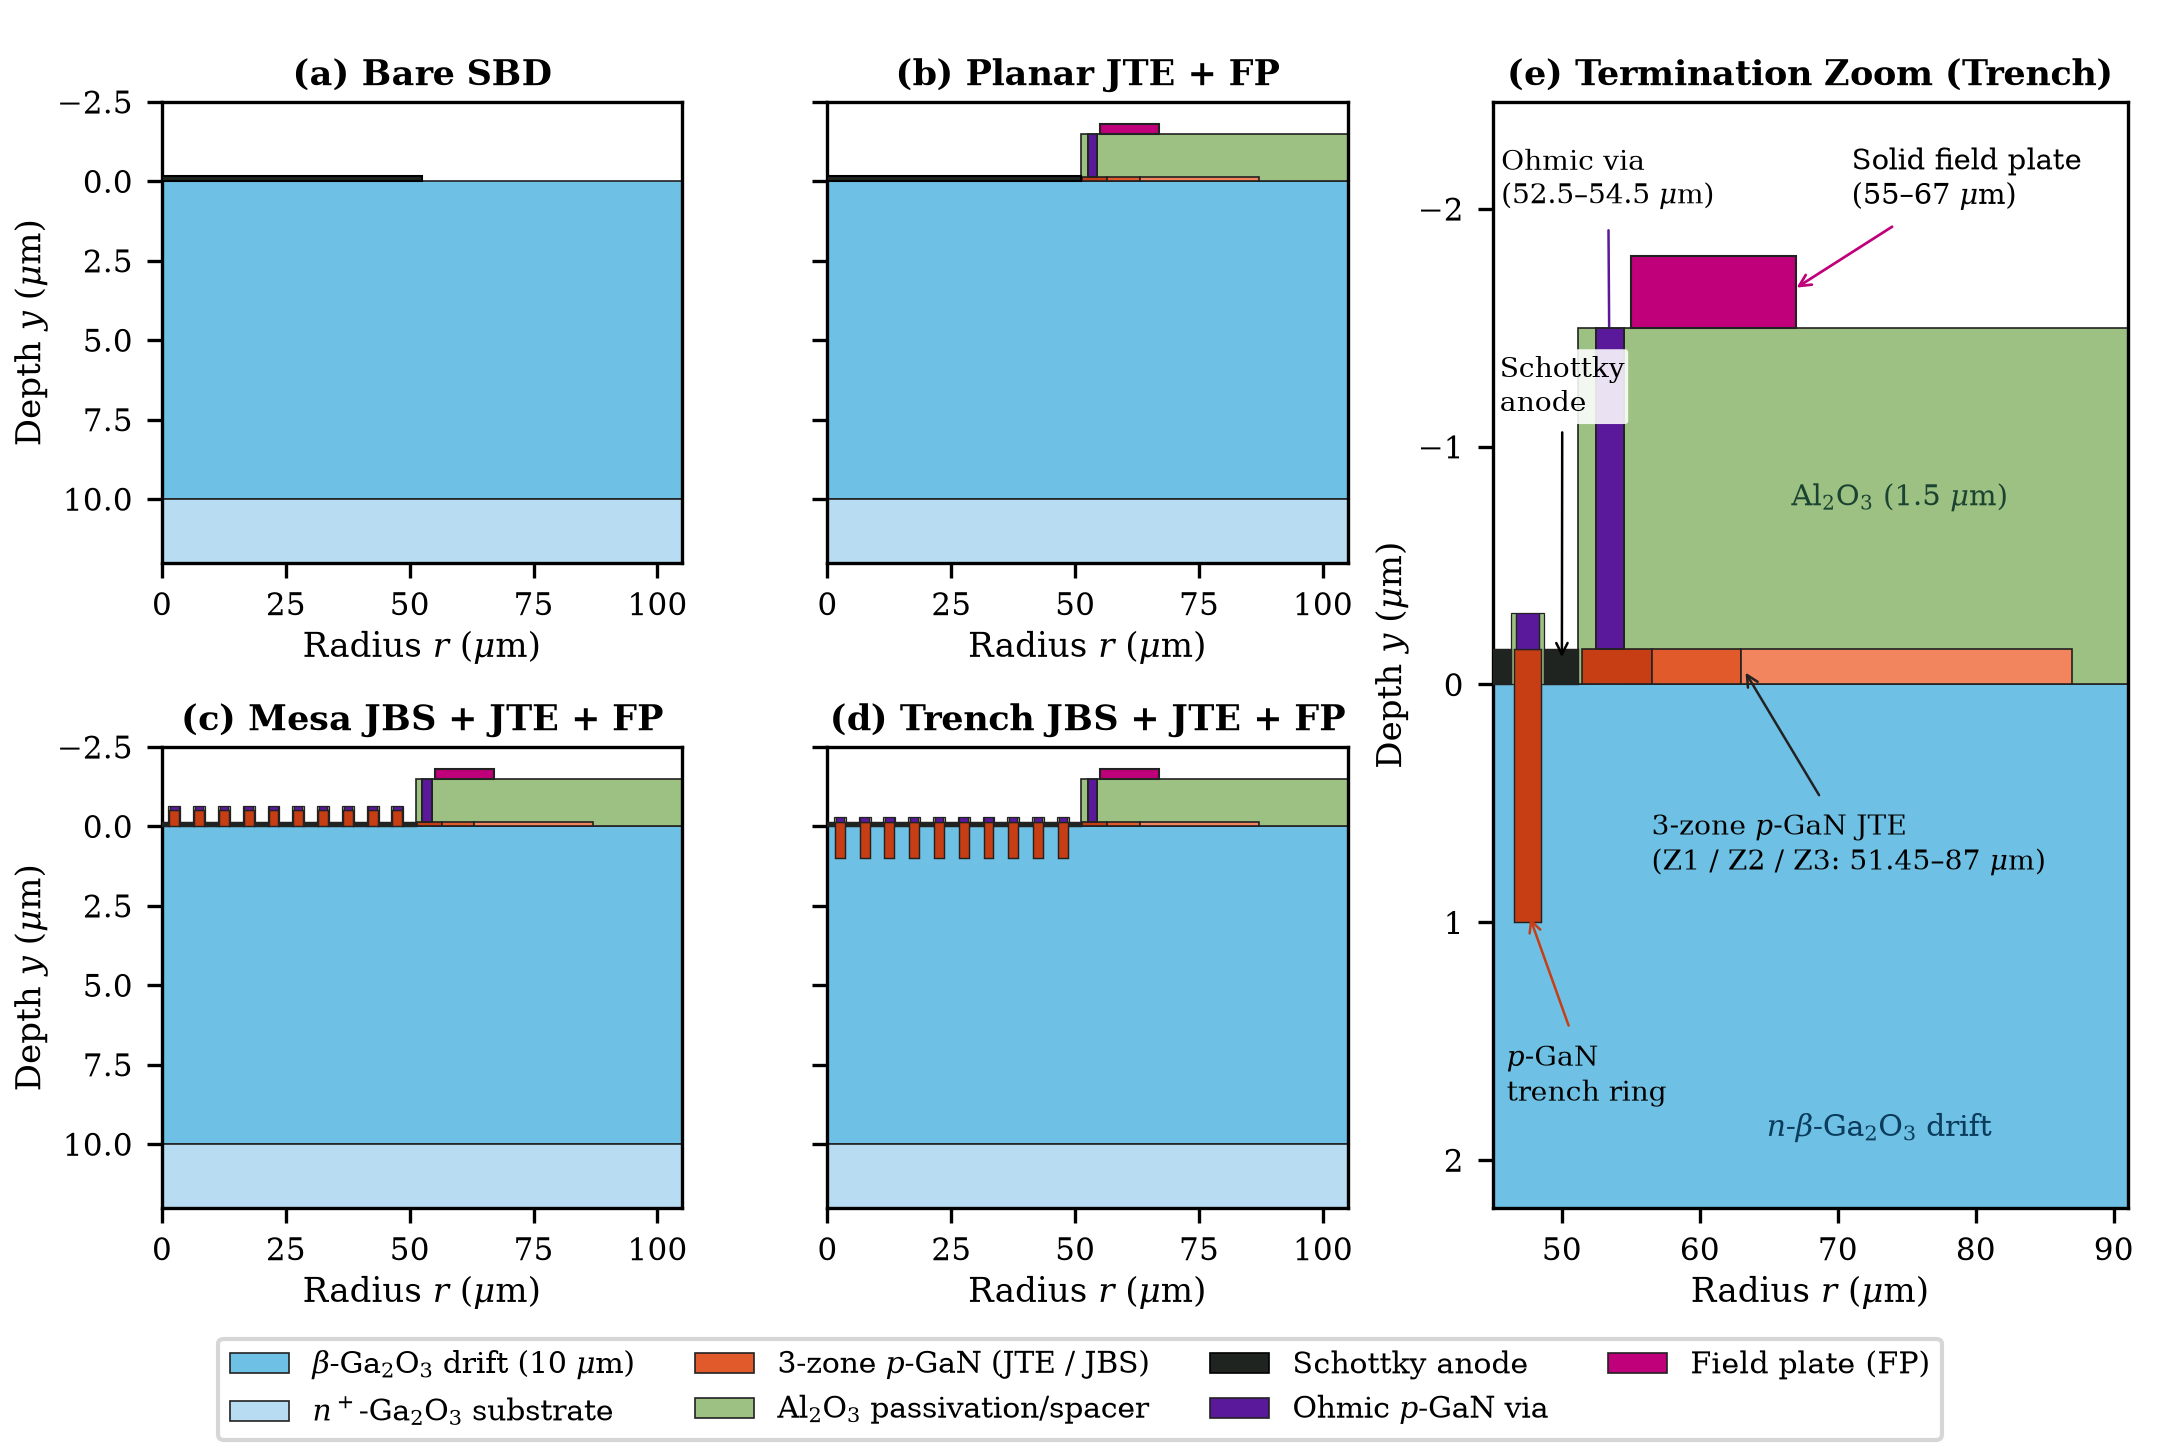
\includegraphics[width=0.58\textwidth]{structures.png}
\caption{Schematic cross-sections of the four representative geometries, drawn from the simulated geometry definitions: (a) bare Schottky diode, (b) planar JTE with field plate, (c) mesa JBS with JTE and field plate, (d) trench JBS with JTE and field plate, and (e) enlarged termination view showing the outer \pGaN{} trench ring, Schottky anode, three-zone JTE, Al$_2$O$_3$ spacer and Al field plate. Only the upper part of the substrate is shown; the terminated devices extend laterally to 135~$\mu$m, and the vertical axis is the mesh coordinate $y$, which is negative above the epi surface. The no-FP cases omit the field-plate electrode from the corresponding geometry.}
\label{fig:structures}
\end{figure*}

\begin{figure*}[!p]
\centering
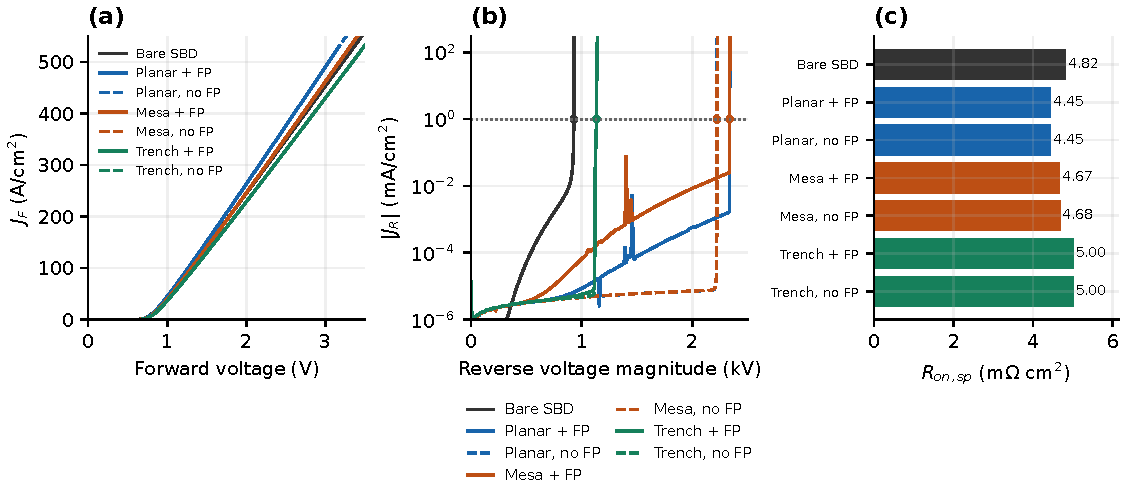
\includegraphics[width=0.66\textwidth]{electrical.pdf}
\caption{Architecture comparison at 298.15~K: (a) forward characteristics, (b) reverse characteristics with markers at the sustained 1~mA/cm$^2$ crossings, and (c) specific resistance from the forward fits over 200--300~A/cm$^2$. The field-plated and unplated curves can overlap.}
\label{fig:electrical}
\end{figure*}

\begin{figure*}[!p]
\centering
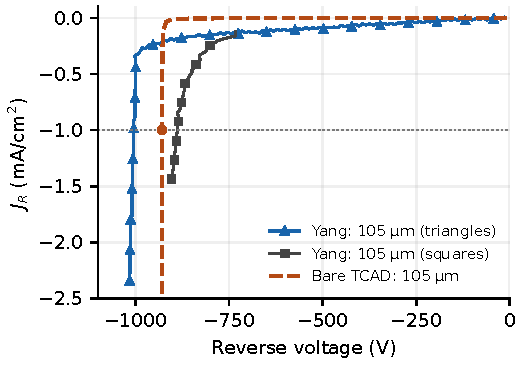
\includegraphics[width=0.38\textwidth]{bare_yang_benchmark.pdf}
\caption{Room-temperature reverse-current benchmark for the 105-$\mu$m bare diode. The triangle and square traces are digitized from Fig.~5 of Yang \emph{et al.}~\cite{Yang2017}; the square trace is shown only where it can be distinguished from overlapping curves. The dashed curve is the selected split-anode TCAD result. The dotted line marks $|J_R|=1$~mA/cm$^2$.}
\label{fig:bare_yang_benchmark}
\end{figure*}

\begin{figure*}[!t]
\centering
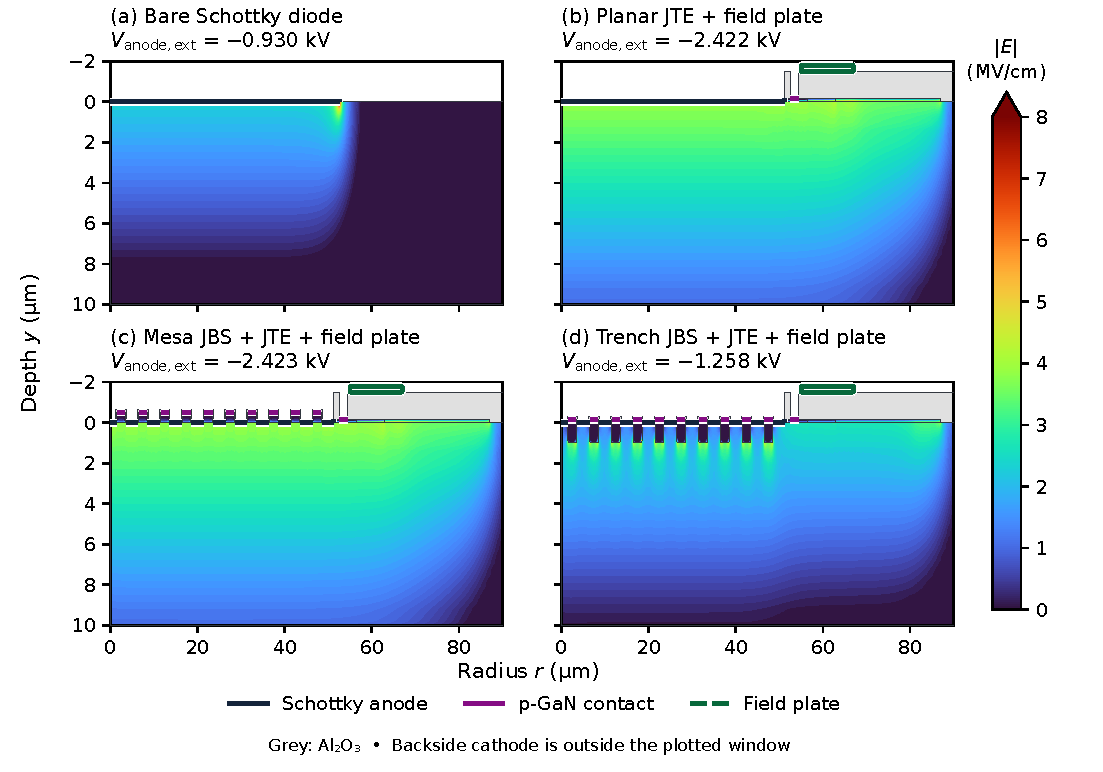
\includegraphics[width=0.91\textwidth]{architecture_reverse_fields.pdf}
\caption{Reverse electric-field magnitude in (a) the bare Schottky diode, (b) the planar JTE with field plate, (c) the mesa JBS with JTE and field plate, and (d) the trench JBS with JTE and field plate. Each panel shows its final saved reverse state at the indicated external anode bias, not a common-bias or current-threshold state. The shared semiconductor scale is 0--8~MV/cm, with values above 8~MV/cm saturated. Grey denotes Al$_2$O$_3$; lines identify the mesh contact boundaries.}
\label{fig:architecture_reverse_fields}
\end{figure*}

\subsection{Forward and reverse characteristics}
Fig.~\ref{fig:electrical} and Table~\ref{tab:architectures} compare the architectures at 298.15~K. The selected bare trace crosses 1~mA/cm$^2$ at 929~V. Figure~\ref{fig:bare_yang_benchmark} compares this trace with two digitized 105-$\mu$m measurements from Yang \emph{et al.}~\cite{Yang2017}. At the same current-density criterion the simulation lies between the two measured traces. The comparison checks the scale of the reverse-current rise, not the agreement of the pre-knee leakage or mesh convergence. The simulated planar and mesa cases cross at approximately 2336~V with a field plate and 2221~V without one. The trench cases reach about 1133~V with or without the plate.

\begin{table*}[!t]
\caption{Extracted Performance at 298.15~K on the Common Reference Area}
\label{tab:architectures}
\centering\footnotesize
\begin{tabular}{lrrrrrr}
\toprule
Structure & $\Von$ (V) & $V_{F,100}$ (V) & $\Ron$ (m$\Omega$\,cm$^2$) & $\Vop$ (V) & $M_{\mathrm{on}}$ (MV) & $B$ (GW/cm$^2$)\\
\midrule
Bare SBD & 0.697 & 1.294 & 4.82 & 929 & 1.24 & 0.179\\
Planar JTE + FP & 0.701 & 1.265 & 4.45 & 2336 & 7.78 & 1.227\\
Planar JTE, no FP & 0.703 & 1.265 & 4.45 & 2221 & 7.02 & 1.109\\
Mesa JBS + JTE + FP & 0.718 & 1.308 & 4.67 & 2336 & 7.60 & 1.167\\
Mesa JBS + JTE, no FP & 0.721 & 1.308 & 4.68 & 2221 & 6.84 & 1.055\\
Trench JBS + JTE + FP & 0.723 & 1.345 & 5.00 & 1133 & 1.78 & 0.257\\
Trench JBS + JTE, no FP & 0.721 & 1.345 & 5.00 & 1133 & 1.78 & 0.257\\
Thin planar, 80 nm, 0.75 eV & 0.355 & 0.916 & 4.45 & 2347 & 15.50 & 1.237\\
\bottomrule
\end{tabular}
\par\smallskip\begin{minipage}{0.96\textwidth}\footnotesize
The last row uses an 80-nm JTE and a 0.75-eV input barrier. The other terminated cases use a 150-nm outer JTE and a 1.10-eV input barrier. The 929-V bare value is from the selected split-anode current trace; the separate corner-mesh study is shown in Fig.~\ref{fig:mesh}. The bare and terminated designs use the same nominal drift and substrate doping but differ in lateral geometry and contact configuration. $R_{\mathrm{on,sp}}$ is compared on the common $A_{\mathrm{ref}}$ only, and the difference between the bare and planar values is not attributed to the termination.
\end{minipage}
\end{table*}

On the meshes used, the planar and mesa field-plated designs reach approximately the same room-temperature current-threshold voltage. The mesa case has a smaller exposed Schottky area and a higher fitted resistance on the common reference area.

In the tested trench designs the 1~mA/cm$^2$ crossing is near 1133~V and is nearly unchanged between the plated and unplated variants. This is a comparison of the specified designs, not an isolated test of recessing otherwise identical active junctions.

Within the terminated designs, the fitted resistance on $A_{\mathrm{ref}}$ increases from the planar to the mesa and trench cases (Table~\ref{tab:architectures}). The selected bare reference is listed separately.

Figure~\ref{fig:architecture_reverse_fields} shows the reverse electric-field distribution of the four representative devices at their final saved biases.

\subsection{\pGaN{} thickness and acceptor concentration}
\begin{figure}[!t]
\centering
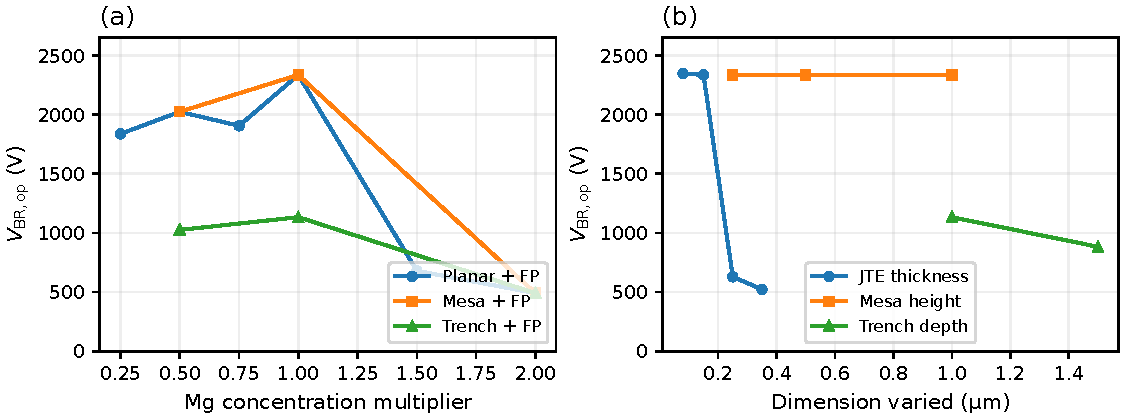
\includegraphics[width=\columnwidth]{geometry_sensitivity_v6.pdf}
\caption{Operational blocking voltage versus (a) prescribed Mg concentration multiplier and (b) varied dimension. The mesa spacer height changes with the mesa height. Lines connect simulated points; they do not define a continuous process window.}
\label{fig:geometry}
\end{figure}

Figure~\ref{fig:geometry}(a) shows the response to changing the prescribed Mg concentration. In the planar JTE with FP, the largest crossing among the sampled multipliers occurs at the nominal dose. It falls from 2336 to 680~V at $1.5\times$ dose. The lower doses do not follow a monotonic trend, so the tested points do not establish a continuous process window.

The mesa and trench results are shown at their sampled dose multipliers only. In particular, the lower-dose response of the trench does not follow the planar sequence.

For the planar JTE with FP, thicknesses of 0.08, 0.15, 0.25 and 0.35~$\mu$m give 2347, 2336, 629 and 524~V at the nominal input barrier. The largest drop among these cases occurs between 150 and 250~nm. The low-barrier 80-nm case is a separate design point. Raising the mesa from 0.25 to 1.00~$\mu$m while increasing spacer height from 0.40 to 1.15~$\mu$m leaves the threshold near 2336~V. Increasing trench depth from 1.00 to 1.50~$\mu$m changes the threshold from 1133 to 883~V in the tested trench designs.

\begin{figure*}[!t]
\centering
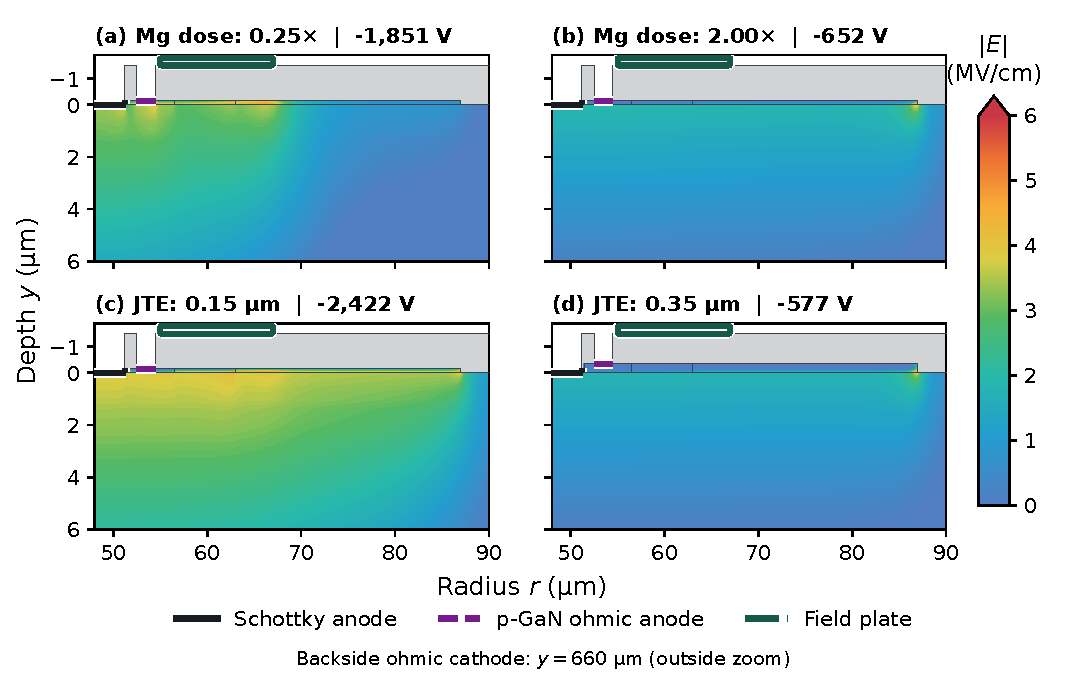
\includegraphics[width=0.78\textwidth]{reverse_field_contacts.pdf}
\caption{Reverse electric-field magnitude in the planar JTE with field plate. Top: 0.25$\times$ and 2.00$\times$ nominal Mg dose at 0.15~$\mu$m JTE thickness. Bottom: 0.15 and 0.35~$\mu$m JTE thickness at nominal dose. Panel titles give the saved external anode voltages, not the blocking crossings. The semiconductor uses a shared 0--6~MV/cm linear scale, with values above 6~MV/cm shown in the top colour. Grey denotes Al$_2$O$_3$.}
\label{fig:fields}
\end{figure*}

Figure~\ref{fig:fields} shows the reverse electric field across the planar termination for selected dose and thickness cases. Each panel is at its own final saved reverse bias. The maps illustrate where the field is concentrated; they do not quantify field reduction at a common voltage.

Fig.~\ref{fig:bands}(a),(b) shows equilibrium band cuts at $r=60~\mu$m for selected dose and thickness variants. The model uses electron affinities of 4.00~eV for \GaO{} and 3.922~eV for GaN, a 0.078~eV conduction-band offset, with a corresponding valence-band offset of about 1.4~eV; the solved band gaps at 298~K are 4.80 and 3.44~eV. Because the \pGaN{} termination is much more heavily doped than the $2.0\times10^{16}$~cm$^{-3}$ drift layer, the zero-bias band bending drops almost entirely in the \GaO{} drift, and the equilibrium curves for different dose and thickness overlap closely. The strong reverse-bias sensitivity in Fig.~\ref{fig:bands}(c),(d) is consistent with changes in depletion and charge balance under reverse bias; the final-state cuts are not a comparison at a common voltage.

\begin{figure*}[!t]
\centering
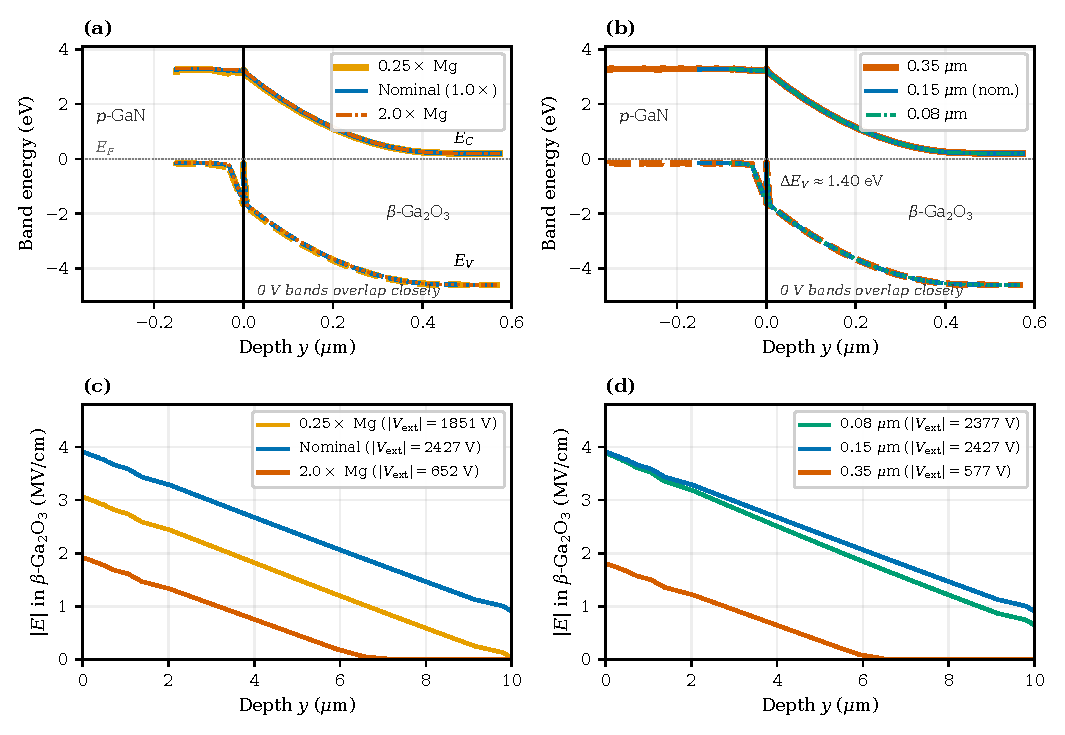
\includegraphics[width=0.78\textwidth]{bands_fields.pdf}
\caption{Cutlines at $r=60~\mu$m: (a),(b) 0-V band diagrams versus Mg multiplier and termination thickness, with solid $E_C$ and dashed $E_V$ referenced to $E_F=0$; the curves overlap closely because the built-in band bending falls mainly in the lightly doped drift. (c),(d) Reverse drift-region field profiles at the final saved reverse-bias states, which need not be at the same voltage. In (b) and (d) the 0.08-$\mu$m curve is the 80-nm, 0.75-eV design point; it is not a member of the 1.10-eV thickness series, and it differs in both thickness and input barrier from the 150-nm reference. The annotated state voltages are the solver's final applied voltages.}
\label{fig:bands}
\end{figure*}

\subsection{Schottky barrier height}
Figure~\ref{fig:barrier} varies the input barrier across 0.75--1.50~eV. The planar blocking crossing stays near 2336~V while its turn-on voltage decreases from 0.701 to 0.354~V between 1.10 and 0.75~eV. The trench crossing remains near 1.13~kV. The mesa crossing falls from about 2336 to 2061~V at 0.75~eV.

Lowering the barrier has a second cost. At $-1$~kV the planar leakage rises from $8.6\times10^{-9}$ to $1.10\times10^{-4}$~A/cm$^2$ between 1.10 and 0.75~eV, so the 0.1~mA/cm$^2$ threshold falls from 2335~V to 926~V for the 150-nm case, and to 925~V for the 80-nm design of Table~\ref{tab:architectures}; these are two different devices under the same leakage criterion. The choice of barrier is therefore a trade against the leakage specification even when the crossing at a higher current criterion changes little.

\begin{figure*}[!t]
\centering
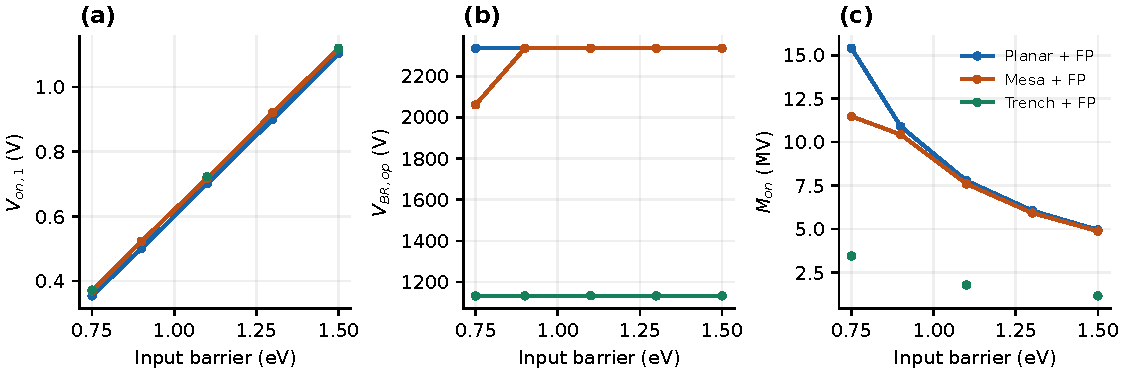
\includegraphics[width=0.86\textwidth]{barrier.pdf}
\caption{Input-barrier sweep at 298.15~K: (a) turn-on at 1~A/cm$^2$, (b) blocking at 1~mA/cm$^2$, and (c) $M_{\mathrm{on}}$. Two incomplete trench forward sweeps at 0.90 and 1.30~eV are omitted from (a) and (c); their valid reverse crossings are included in (b).}
\label{fig:barrier}
\end{figure*}

\subsection{Temperature}
\begin{figure}[!t]
\centering
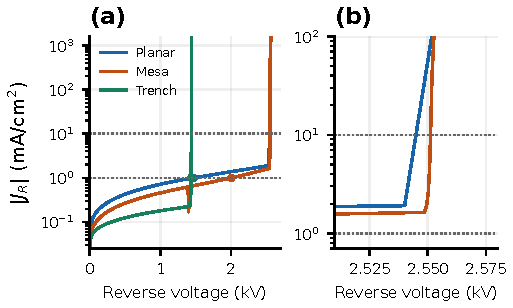
\includegraphics[width=\columnwidth]{reverse_400K.pdf}
\caption{Simulated reverse current density at 400~K: (a) full comparison with markers at the sustained 1~mA/cm$^2$ crossings; (b) zoom near the steep rise in the planar and mesa currents. Dotted lines indicate the 1 and 10~mA/cm$^2$ criteria.}
\label{fig:temperature}
\end{figure}

Fig.~\ref{fig:temperature} compares the terminated families at 400~K. From 298 to 350~K, the planar crossing shifts from about 2336~V to a bracket of 2430--2446~V. This shift to higher voltage and the steep, sustained rise in hole current are consistent with avalanche in the \pGaN{} termination. At 400~K, the planar and mesa devices reach 1~mA/cm$^2$ on the electron-leakage branch, at about 1473 and 2007~V, respectively. The mesa crosses at 2440~V at 350~K, and the trench crossings at 298, 350 and 400~K are 1133, 1280 and 1438~V, respectively.

At the planar 400-K crossing, the calculated reverse current is dominated by the Schottky electron component. The mesa has 54.2\% of the planar exposed Schottky area, but its leakage per unit of that area is higher at matched bias. Thus the higher mesa voltage at this common-reference current criterion may partly reflect the smaller exposed area and does not establish better local leakage suppression.

At 10~mA/cm$^2$ and 400~K, the planar and mesa crossings are 2545 and 2551~V, while the trench crosses at 1439~V. The planar and mesa cross this higher criterion on the steep rise into the hole-dominated branch. Their sample brackets overlap (2540.1--2555.6 and 2550.8--2551.2~V), so the order of their crossings is not resolved.
\subsection{Best structure and comparison with published devices}
Among the architecture cases in Table~\ref{tab:architectures}, the 80-nm planar JTE at a 0.75-eV input barrier gives the highest $M_{\mathrm{on}}$. The main difference from the 150-nm, 1.10-eV case is its lower turn-on voltage; the simulated 1~mA/cm$^2$ blocking voltages and Baliga figures of merit remain close.

\begin{table*}[!t]
\caption{Comparison with Published Rectifiers}
\label{tab:literature}
\centering\scriptsize
\setlength{\tabcolsep}{2.2pt}
\begin{tabular}{>{\raggedright\arraybackslash}p{2.1cm}lrrrrr}
\toprule
Device & Evidence & $V_{\mathrm{BR}}$ (V) & $V_{\mathrm{on}}$ (V) & $\Ron$ (m$\Omega$\,cm$^2$) & $V^2/V_{\mathrm{on}}$ (MV) & $B$ (GW/cm$^2$)\\
\midrule
Yang \emph{et al.}~\cite{Yang2017} & measured & $975\pm40$ & -- & $\sim$6.7 & -- & 0.154$^{a}$\\
Su \emph{et al.}~\cite{Su2024_APL} & measured & 2340 & 0.64 & 5.3 & 8.56 & 1.03\\
Chang \emph{et al.}~\cite{Chang2025_APL} & measured & 3000$^{b}$ & 0.80 & 6.15 & 11.25 & 1.46\\
Planar JTE + FP, 0.15~$\mu$m, 1.10~eV & simulated & 2336 & 0.701 & 4.45 & 7.78 & 1.227\\
Planar JTE + FP, 0.08~$\mu$m, 0.75~eV & simulated & 2347 & 0.355 & 4.45 & 15.50 & 1.237\\
\bottomrule
\end{tabular}
\par\smallskip\begin{minipage}{0.98\columnwidth}\footnotesize
$^{a}$Author-reported value. $^{b}$Measured at a reverse current density of 1~A/cm$^2$~\cite{Chang2025_APL}. Simulated reverse voltages use 1~mA/cm$^2$ on $A_{\mathrm{ref}}$. Literature values retain their original extraction conventions.
\end{minipage}
\end{table*}

The same 80-nm, 0.75-eV case crosses 0.1~mA/cm$^2$ at 925~V, compared with 2347~V at 1~mA/cm$^2$. The lower turn-on voltage therefore comes with a substantial reverse-leakage trade-off when the current limit is tightened.

Table~\ref{tab:literature} places the simulated values alongside reported measurements. The table is not a ranking at a common reverse-current criterion. In particular, Chang \emph{et al.} report 3~kV at 1~A/cm$^2$~\cite{Chang2025_APL}, while this study reports simulation crossings at 1~mA/cm$^2$.

\section{Design Sensitivity and Limitations}
The strongest sensitivity in the planar cases is to the prescribed \pGaN{} thickness and acceptor concentration. Increasing the thickness from 150 to 250~nm lowers the crossing from 2336 to 629~V, and increasing Mg concentration to $1.5\times$ nominal lowers it to 680~V. These are changes between sampled simulation points, not manufacturing tolerances. The nearly unchanged mesa crossing applies to the paired ring and spacer height changes, not to either dimension independently.

Chang \emph{et al.} demonstrated a sputtered \pGaN/\GaO{} termination~\cite{Chang2025_APL}; that process does not validate the exact three-zone profile or the bulk-GaN ionisation coefficients used here. The equilibrium ionised fraction is a model output, not a measured process activation fraction. The 1.5-$\mu$m Al$_2$O$_3$ model uses $\varepsilon_r=9$ and assumed interface charge; it does not include dielectric failure. The Schottky and spacer-foot fillets are nominal model dimensions. Contact and dielectric reliability, trap-assisted leakage beyond the included models, and self-heating were not validated.

\section{Conclusion}
The nominal plated planar and mesa designs in this TCAD study reach about 2336~V at 1~mA/cm$^2$, compared with 1133~V for the tested trench and 929~V for the selected bare reference. The pronounced drop from 2336 to 629~V when planar JTE thickness increases from 150 to 250~nm illustrates why the termination profile matters. At 400~K, the planar and mesa crossings differ by about 534~V at 1~mA/cm$^2$, but their crossing brackets overlap at 10~mA/cm$^2$. The 80-nm, low-barrier design improves turn-on, but its 925-V crossing at 0.1~mA/cm$^2$ limits the benefit under a stricter leakage specification. These results guide comparisons within the tested design space; they do not establish fabricated voltage ratings.

\section*{Acknowledgment}
The author thanks his project supervisor and research group for technical guidance, and the Microelectronics Laboratory for computational and Synopsys TCAD facilities.

\bibliographystyle{IEEEtran}
\bibliography{references}
\end{document}